\section{Serial Interfaces}
\subsection{Network Toopologies}
Point-to-point, Star, Bus, Ring, Mesh, Line, Tree, Fully Connected

\subsection{LVDS}
Low Voltage Digital Signalling pads are hardware specific. They are marked with ``N'' and ``P'' in Vivado.
\begin{lstlisting}
set_property IOSTANDARD LVDS [get_ports clk_p]
\end{lstlisting}


\subsection{SPI}
Benötigt 3 + \#Slaves Pins und wird max bis 100MHz betrieben. Eine Transaktion starte, wenn CS auf 0 springt.
\begin{center}
	\includegraphics[width=\columnwidth]{Images/spi}
\end{center}
\begin{center}
	\includegraphics[width=\columnwidth]{Images/spi_mode}
\end{center}

\subsection{I$^2$C}
Benötigt zwei \textbf{bidirectionale} Leitungen, unabhängig von Anzahl Slaves und wird zwischen 100kbit/s bis 3.4Mbit/s betrieben. Wichtig dabei, beide Leitungen müssen immer einen Pull-Up Widerstand haben.
\begin{center}
	\includegraphics[width=0.7\columnwidth]{Images/i2c}
\end{center}
\begin{center}
	\includegraphics[width=0.7\columnwidth]{Images/i2c_start}
\end{center}

Timing Übersicht:
\begin{center}
	\includegraphics[width=\columnwidth]{Images/i2c_timing}
\end{center}

\section{Parallel Interface}
\subsection{AXI}
AXI ist ein 1-to-1 Interface (Master-Slave) mit fünf unabhängigen Channels:
\begin{center}
	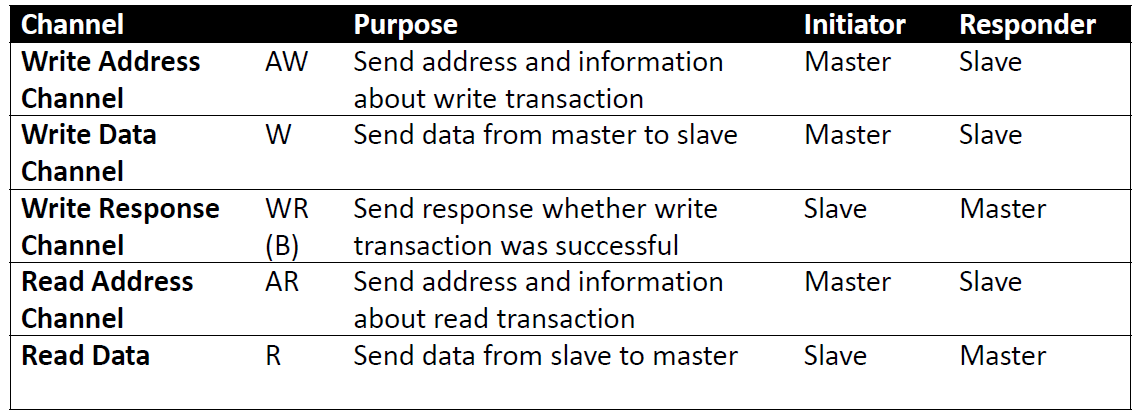
\includegraphics[width=\columnwidth]{Images/axi}
\end{center}

Dabei gibt es drei Unterschiedliche Varianten:
\begin{itemize}
	\item \textbf{AXI4}(-Full), unterstützt BurstMode bis zu 256 Daten Packeten pro Address und ist Memmory Mapped
	\item \textbf{AXI4-Lite}, Keine Burst und ist Memory Mapped für einzelne Transaktionen
	\item \textbf{AXI4-Stream}, Für Streaming Anwendungen und daher nur Schreib-Channel. Nur Daten von Master zu Slave möglich mit unlimitierten Burst grösse.
\end{itemize}

\subsubsection{Interconnect}
Da AXI eine Schnittstelle zwischen Master-Slave ist, wird ein Interconnect für die n-m Kommuikation benötig. Dieser Interconnect entscheided auf basis der Address, zu welchem Slave er die Packete routen muss.
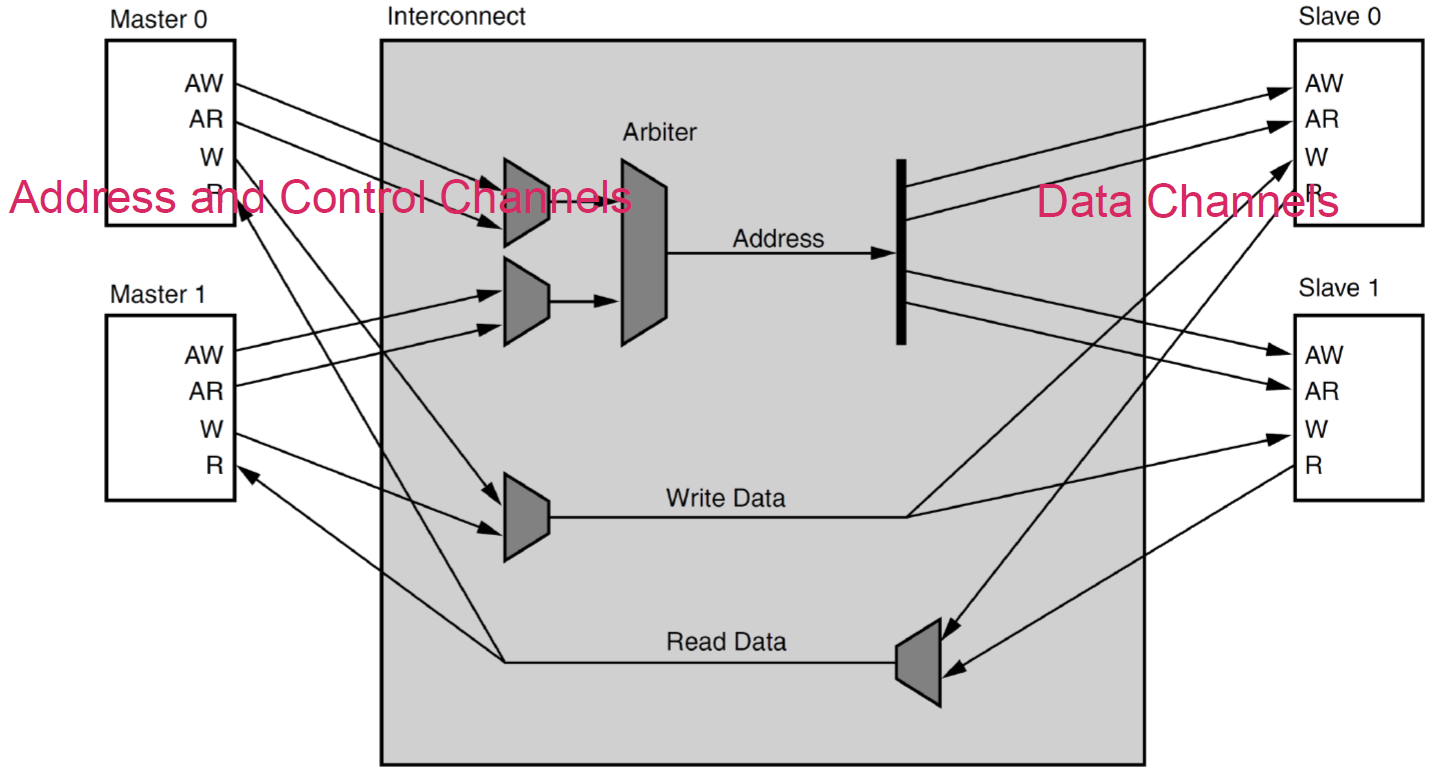
\includegraphics[width=\columnwidth]{Images/interconnect}
